\documentclass[11pt,a4paper]{article}
\usepackage[margin=2.4cm]{geometry}
\usepackage{amsmath,amssymb,amsthm,bm}
\usepackage{booktabs,array,tabularx}
\usepackage{graphicx}
\graphicspath{{figures/}}
\usepackage{xcolor}
\usepackage[hidelinks]{hyperref}
\usepackage{enumitem}
\setlist{itemsep=2pt,topsep=4pt}
\numberwithin{equation}{section}

\newcommand{\qv}{\vec q}
\newcommand{\ket}[1]{|#1\rangle}
\newcommand{\bra}[1]{\langle #1|}
\newcommand{\qh}{\hat q}
\newcommand{\dd}{\mathrm{d}}
\newcommand{\Eth}{E_{\rm th}}
\newcommand{\mchi}{m_\chi}
\newcommand{\avg}[1]{\langle #1\rangle}
\newcommand{\CaWO}{CaWO$_4$}
\newcommand{\AlO}{Al$_2$O$_3$}
\newcommand{\TeO}{TeO$_2$}
\newcommand{\LNO}{LiNbO$_3$}

\title{\textbf{Dark matter and the neutrino background\\ with the full lattice response of cryogenic crystals}\\[4pt]
\large Derivations, implementation and results of the NuFog\,v2 pipeline}
\author{Israel Hern\'andez\\ \small Working report, 29 October 2026}
\date{}

\begin{document}
\maketitle

\begin{abstract}
\noindent
This report documents the calculation of dark matter (DM) discovery limits in the presence of
the coherent elastic neutrino--nucleus scattering (CEvNS) background for crystal targets with
energy thresholds from tens of meV to eV. In that range the recoil energy is absorbed by the
lattice through the emission of one or many phonons, not by a free nucleus. Both the DM signal
and the neutrino background are therefore governed by the dynamic structure factor
$S(\vec q,\omega)$ of the crystal.

All formulas are derived from first principles:
\begin{itemize}
  \item the scattering rate from Fermi's golden rule;
  \item the multiphonon expansion of a harmonic crystal in the incoherent approximation,
  with its sum rules and impulse limit;
  \item the DM and CEvNS rates, the Asimov discovery test with flux nuisance parameters, and
  the scaling laws that distinguish a background from a ``fog'';
  \item the directional (daily-modulation) signal of anisotropic crystals.
\end{itemize}

The implementation and its validation are described. Results are given for CaWO$_4$,
Al$_2$O$_3$, TeO$_2$, LiNbO$_3$ and Si, together with a comparison with CRESST and with the
literature. A final section derives why the lattice response must be known precisely: the
low-mass rate depends on the phonon spectrum as a high power of its moments, and the ability
to separate DM from neutrinos rests on the spectral shape that $S(\vec q,\omega)$ produces.
\end{abstract}

\tableofcontents
\newpage

%==============================================================================
\section{Scope and conventions}
%==============================================================================
We use natural units $\hbar=c=k_B=1$. The DM mass is $\mchi$, the nucleon mass $m_n$, and the
DM--nucleon reduced mass $\mu=\mchi m_n/(\mchi+m_n)$. Atoms in the unit cell are labelled by
$d$, with mass $m_d$, mass number $A_d$, atomic number $Z_d$ and displacement $\vec u_d$.
The momentum transfer is $\qv=q\,\qh$, and the energy deposited in the crystal is $\omega$.
$V$ is the unit-cell volume, $M_{\rm cell}=\sum_d m_d$ the cell mass, and
$\rho_T=M_{\rm cell}/V$ the target mass density.

The analysis assumes:
\begin{itemize}
  \item spin-independent DM--nucleon scattering through a heavy mediator, with equal couplings
  to protons and neutrons;
  \item the Standard Halo Model (SHM) with $\rho_\chi=0.3$\,GeV\,cm$^{-3}$,
  $v_0=220$, $v_E=232$ and $v_{\rm esc}=544$\,km\,s$^{-1}$;
  \item a crystal at zero temperature.
\end{itemize}
The detector response is a threshold $\Eth$ and a Gaussian resolution $\sigma_E=\Eth/5$,
following the CRESST convention.

%==============================================================================
\section{Scattering off a crystal: the dynamic structure factor}
\label{sec:S}
%==============================================================================
\subsection{Rate from Fermi's golden rule}
For a contact interaction, the DM scatters off each nucleus $J$ with an amplitude proportional to its coherent coupling $f_J$ ($f_J=A_J$ for spin-independent scattering) times the nuclear form factor $F_J(q)$. The normalization is chosen such that a single free nucleon has cross section $\sigma_n$. In Born
approximation the transition rate of a DM particle with velocity $\vec v$, which excites the
crystal from its ground state $\ket0$ to a state $\ket f$, is
\begin{equation}
  \Gamma(\vec v) = \frac{\pi\sigma_n}{\mu^2}\int\!\frac{\dd^3q}{(2\pi)^3}\,
  S(\qv,\omega_{\qv}), \qquad
  \omega_{\qv} = \qv\cdot\vec v - \frac{q^2}{2\mchi},
  \label{eq:Gamma}
\end{equation}
where energy conservation fixes the deposited energy $\omega_{\qv}$, and the
\emph{dynamic structure factor} is
\begin{equation}
  S(\qv,\omega) = \frac{2\pi}{V_{\rm tot}}\sum_f
  \Big|\bra f \sum_J f_J F_J(q)\, e^{i\qv\cdot\vec r_J}\ket0\Big|^2
  \delta(E_f-E_0-\omega).
  \label{eq:Sdef}
\end{equation}
Here $V_{\rm tot}$ is the crystal volume. Because $S$ is extensive in the number of cells, it
is convenient to quote it per unit cell, replacing $V_{\rm tot}$ by $V$ and the sum over $J$
by a sum over the atoms $d$ of one cell (Sec.~\ref{sec:incoherent}).

\subsection{Differential rate per unit target mass}
The event rate per unit target mass is
\begin{equation}
  R = \frac{1}{\rho_T}\frac{\rho_\chi}{\mchi}\int \dd^3v\, f(\vec v)\,\Gamma(\vec v).
\end{equation}
Inserting $1=\int\dd\omega\,\delta(\omega-\omega_{\qv})$,
\begin{equation}
  \frac{\dd R}{\dd\omega} = \frac{1}{\rho_T}\frac{\rho_\chi}{\mchi}
  \frac{\pi\sigma_n}{\mu^2}\int\!\frac{\dd^3q}{(2\pi)^3}\,S(\qv,\omega)
  \int\dd^3v\, f(\vec v)\,
  \delta\!\left(\qv\cdot\vec v-\frac{q^2}{2\mchi}-\omega\right).
  \label{eq:dRdw_general}
\end{equation}
The velocity integral defines the \emph{Radon transform} of $f$,
\begin{equation}
  \int\dd^3v\, f(\vec v)\,\delta(\qv\cdot\vec v-q v^*)
  = \frac{1}{q}\, g(v^*,\qh),
  \qquad
  g(w,\qh)\equiv\int\dd^3v\, f(\vec v)\,\delta(\vec v\cdot\qh - w),
  \qquad
  v^* = \frac{q}{2\mchi}+\frac{\omega}{q}.
  \label{eq:radon}
\end{equation}
Here $v^*$ is the minimum velocity component along $\qh$ that can deposit $\omega$ with
momentum $q$.

\paragraph{Isotropic response.}
If $S$ depends only on $q=|\qv|$, the angular integral of $g$ can be done first. Using
$\dd^3q = q^2\dd q\,\dd\Omega_q$ and
\begin{equation}
  \int\frac{\dd\Omega_q}{4\pi}\, g(w,\qh)
  = \int\dd^3v\, f(\vec v)\int\frac{\dd\Omega_q}{4\pi}\,\delta(v\cos\theta - w)
  = \int\dd^3v\,\frac{f(\vec v)}{2v}\,\Theta(v-w)
  \equiv \frac12\,\eta(w),
  \label{eq:g_to_eta}
\end{equation}
where $\eta(v_{\min})=\int\dd^3v\,f(\vec v)\,\Theta(v-v_{\min})/v$ is the mean inverse speed,
one obtains
\begin{equation}
  \boxed{\;
  \frac{\dd R}{\dd\omega} = \frac{1}{\rho_T}\frac{\rho_\chi}{\mchi}
  \frac{\sigma_n}{4\pi\mu^2}\int q\,\dd q\;\eta(v^*)\,S(q,\omega)\;}
  \label{eq:dRdw}
\end{equation}
The steps are
$\frac{\pi}{(2\pi)^3}\cdot 4\pi\cdot\frac{1}{2}=\frac{1}{4\pi}$, with one power of $q$
cancelled by Eq.~\eqref{eq:radon}. The $q$ integral runs up to
$q_{\max}=2\mchi(v_{\rm esc}+v_E)$.

\subsection{Free-nucleus limit (consistency check)}
For a free nucleus of mass $M$ and coupling $A$, Eq.~\eqref{eq:Sdef} per nucleus gives
$S=(2\pi/V)A^2F^2\,\delta(\omega-q^2/2M)$. Using
$\int q\,\dd q\,\delta(\omega-q^2/2M)=M$ and $1/(\rho_T V)=1/M_{\rm cell}$ (one nucleus per
``cell''),
\begin{equation}
  \frac{\dd R}{\dd E_R} = \frac{\rho_\chi}{\mchi}\,
  \frac{\sigma_n A^2 F^2(q)}{2\mu^2}\,\eta(v_{\min}),
  \qquad v_{\min}=\sqrt{\frac{M E_R}{2\mu_{\chi N}^2}}.
\end{equation}
This is the textbook rate per nucleus. The pipeline reproduces it numerically to 0.1\% for all
five materials (Sec.~\ref{sec:validation}).

%==============================================================================
\section{The harmonic crystal}
\label{sec:harmonic}
%==============================================================================
\subsection{Phonons and the density-of-states tensor}
Write the position of atom $d$ in cell $\ell$ as
$\vec r_{\ell d}=\vec R_\ell+\vec x_d+\vec u_{\ell d}$. In the harmonic approximation,
\begin{equation}
  \vec u_{\ell d} = \sum_{\nu,\vec k}\frac{1}{\sqrt{2N m_d\,\omega_{\nu\vec k}}}
  \left(\vec e_{d,\nu\vec k}\,a_{\nu\vec k}\,e^{i\vec k\cdot\vec R_\ell} + \text{h.c.}\right),
\end{equation}
where $\omega_{\nu\vec k}$ and $\vec e_{d,\nu\vec k}$ are the frequencies and eigenvector
components of the $3n$ branches, $N$ is the number of cells, and the eigenvectors satisfy the
completeness relation $\sum_\nu e^{i*}_{d,\nu\vec k}e^{j}_{d,\nu\vec k}=\delta^{ij}$ for each
atom $d$. We define the \emph{per-atom density-of-states (DOS) tensor}
\begin{equation}
  D^{ij}_d(\omega) = \frac1N\sum_{\nu,\vec k} e^{i*}_{d,\nu\vec k}\,e^{j}_{d,\nu\vec k}\,
  \delta(\omega-\omega_{\nu\vec k}),
  \qquad \int\dd\omega\, D^{ij}_d = \delta^{ij},
\end{equation}
and its projection along $\qh$,
\begin{equation}
  D_d^{\qh}(\omega) = \qh_i\, D^{ij}_d(\omega)\,\qh_j,
  \qquad \int\dd\omega\, D_d^{\qh}=1 .
\end{equation}
The scalar (isotropic) DOS is $\frac13{\rm Tr}\,D_d$. The tensor is computed from
first-principles force constants (phonopy) on a dense $\vec k$ mesh without symmetry
reduction, with the non-analytic LO--TO correction when Born charges are available.

\subsection{Incoherent approximation}
\label{sec:incoherent}
Expanding $|\sum_J\ldots|^2$ in Eq.~\eqref{eq:Sdef} produces terms with $J=J'$ and
interference terms $J\neq J'$. For $q\gg 2\pi/a$, with $a$ the interatomic distance
(a few keV), the interference terms average out. Keeping only $J=J'$ gives
\begin{equation}
  S(\qv,\omega) = \frac{2\pi}{V}\sum_{d\in{\rm cell}} f_d^2 F_d^2(q)\; S_d(\qv,\omega),
  \qquad
  S_d(\qv,\omega)=\sum_f\big|\bra f e^{i\qv\cdot\vec u_d}\ket 0\big|^2
  \delta(E_f-E_0-\omega).
  \label{eq:Sincoh}
\end{equation}
This approximation fails at the lowest momentum transfers, where single-phonon scattering is
coherent and depends on the phonon dispersion. That affects masses below about 1\,MeV and
the directional signal (Sec.~\ref{sec:directional}).

\subsection{Correlation function and Debye--Waller factor}
Writing the energy $\delta$-function as a time integral and using the Heisenberg picture,
\begin{equation}
  S_d(\qv,\omega)=\int_{-\infty}^{\infty}\frac{\dd t}{2\pi}\,e^{i\omega t}\,
  \big\langle e^{-i\qv\cdot\vec u_d(0)}\,e^{i\qv\cdot\vec u_d(t)}\big\rangle .
\end{equation}
For a harmonic system, $X\equiv\qv\cdot\vec u_d$ is linear in Gaussian (bosonic) operators,
so Bloch's identity
$\avg{e^{-iX(0)}e^{iX(t)}}=e^{-\avg{X^2}}\,e^{\avg{X(0)X(t)}}$ holds. At $T=0$,
\begin{equation}
  \avg{X(0)X(t)} = \sum_{\nu\vec k}\frac{|\qv\cdot\vec e_{d,\nu\vec k}|^2}
  {2N m_d\,\omega_{\nu\vec k}}\,e^{-i\omega_{\nu\vec k}t}
  = \frac{q^2}{2m_d}\int\dd\omega'\,\frac{D_d^{\qh}(\omega')}{\omega'}\,e^{-i\omega' t}.
  \label{eq:XX}
\end{equation}
At $t=0$ this defines the Debye--Waller exponent
\begin{equation}
  2W_d(\qv)\equiv\avg{X^2}=\frac{q^2}{2m_d}\,\avg{\frac1\omega}_{\!d}^{\qh},
  \qquad
  \avg{\frac1\omega}_{\!d}^{\qh}\equiv\int\dd\omega\,\frac{D_d^{\qh}(\omega)}{\omega},
  \qquad
  W_d=\frac{q^2}{4m_d}\avg{\frac1\omega}_{\!d}^{\qh}.
\end{equation}

\subsection{Multiphonon expansion}
Expanding $e^{\avg{X(0)X(t)}}$ in powers and Fourier transforming term by term,
\begin{equation}
  \boxed{\;S_d(\qv,\omega) = e^{-2W_d(\qv)}\sum_{n=0}^{\infty}\frac{1}{n!}
  \left(\frac{q^2}{2m_d}\right)^{\!n} T_{d,n}(\omega),\qquad
  T_{d,1}(\omega)=\frac{D_d^{\qh}(\omega)}{\omega},\quad
  T_{d,n}=T_{d,1}*T_{d,n-1}\;}
  \label{eq:multiphonon}
\end{equation}
with $T_{d,0}=\delta(\omega)$ (the elastic term). The convolution follows from
\begin{equation}
  \int\frac{\dd t}{2\pi}e^{i\omega t}\Big[\int\dd\omega'\,T_1(\omega')e^{-i\omega't}\Big]^n
  = \int\prod_{k=1}^n\dd\omega_k\,T_1(\omega_k)\;\delta\!\Big(\omega-\sum_k\omega_k\Big)
  = T_n(\omega).
\end{equation}
So the $n$-th term is the emission of exactly $n$ phonons. In the code the series is summed
for $n\ge1$ (the elastic term deposits no energy), up to $n_{\max}=60$. The $T_n$ are
computed by FFT convolution on a uniform grid up to 3\,eV.

\subsection{Poisson form and sum rules}
\label{sec:poisson}
Define the normalized single-phonon distribution and the mean phonon number
\begin{equation}
  \hat T_1(\omega)=\frac{T_1(\omega)}{\avg{1/\omega}},\quad\int\hat T_1=1;
  \qquad
  \lambda_d\equiv 2W_d=\frac{q^2}{2m_d}\avg{\frac1\omega}.
\end{equation}
Since $T_n=\avg{1/\omega}^n\hat T_n$ with $\hat T_n$ the $n$-fold convolution of $\hat T_1$,
Eq.~\eqref{eq:multiphonon} becomes
\begin{equation}
  \boxed{\;S_d(\qv,\omega)=\sum_{n\ge0}\underbrace{e^{-\lambda_d}\frac{\lambda_d^n}{n!}}
  _{\text{Poisson}(n;\lambda_d)}\;\hat T_{d,n}(\omega)\;}
  \label{eq:poisson}
\end{equation}
The number of emitted phonons is Poisson-distributed with mean $\lambda_d$, and each phonon
carries an energy drawn from $\hat T_1$. Two exact sum rules follow at once:
\begin{align}
  \int\dd\omega\,S_d &= \sum_n {\rm Pois}(n;\lambda)=1,
  &&\Rightarrow\ \int\dd\omega\sum_{n\ge1}(\ldots)=1-e^{-2W_d},
  \label{eq:sum0}\\
  \int\dd\omega\,\omega\,S_d &= \avg{n}\,\avg{\omega}_{\hat T_1}
  = \lambda_d\cdot\frac{1}{\avg{1/\omega}} = \frac{q^2}{2m_d},
  && \text{(f-sum rule)}.
  \label{eq:fsum}
\end{align}
Here $\avg{\omega}_{\hat T_1}=\int\omega\,T_1/\avg{1/\omega}=1/\avg{1/\omega}$ because
$\int D=1$. The f-sum rule states that, on average, the lattice absorbs exactly the
free-recoil energy $q^2/2m_d$. These identities hold only if $W_d$ and $T_{d,1}$ are built
from the same $D_d$. Their violation was the main defect of the v1 code
(Sec.~\ref{sec:fixes}).

\subsection{Impulse approximation}
For large $q$ the phonon number $\lambda_d$ is large and the sum is dominated by
$n\approx\lambda_d$. Expanding Eq.~\eqref{eq:XX} at short times,
$e^{-i\omega't}\simeq1-i\omega't-\frac12\omega'^2t^2$, gives
\begin{equation}
  \avg{X(0)X(t)}-\avg{X^2}\simeq -i\frac{q^2}{2m_d}t-\frac{q^2\avg{\omega}_d}{4m_d}t^2,
  \qquad \avg\omega_d=\int\omega D_d^{\qh}\,\dd\omega .
\end{equation}
Its Fourier transform is a Gaussian:
\begin{equation}
  S_d(q,\omega)\simeq\frac{1}{\sqrt{2\pi\Delta_d^2}}\exp\!\left[-\frac{(\omega-q^2/2m_d)^2}{2\Delta_d^2}\right],
  \qquad \Delta_d^2=\frac{q^2\avg{\omega}_d}{2m_d}.
\end{equation}
It is centred on the free-nucleus recoil energy and broadened by the zero-point motion. As
$q\to\infty$ it tends to $\delta(\omega-q^2/2m_d)$, the free-nucleus result. The code
switches from Eq.~\eqref{eq:multiphonon} to the Gaussian at $\lambda_d=16$, i.e.\
$q_{\rm thr}=4\sqrt{2m_d\,\bar\omega_{0,d}}$ with $\bar\omega_{0,d}=1/\avg{1/\omega}_d$.

\subsection{Infrared regularization}
The tensor is built with Gaussian smearing ($\sigma=0.5$\,meV), so the numerical $D(\omega)$
is finite at $\omega\to0$. Then $D/\omega$ diverges logarithmically, and $\avg{1/\omega}$
depends on the grid. A real crystal has acoustic modes with $D\propto\omega^2$ (Debye).
Below $\omega_c=2$\,meV the DOS is therefore replaced by
$D(\omega_c)(\omega/\omega_c)^2$, continuously matched and renormalized to unit integral.
$\avg{1/\omega}$, $\avg{\omega}$ and every $T_n$ are then computed from the same regularized
$T_1$, so Eqs.~\eqref{eq:sum0}--\eqref{eq:fsum} hold by construction (to about 1\%
numerically).

\subsection{Couplings, form factor and cell normalization}
For SI DM, $f_d=A_d$. For CEvNS, $f_d=Q_{W,d}=N_d-(1-4\sin^2\theta_W)Z_d$, with
$\sin^2\theta_W=0.23857$. The Helm form factor is
\begin{equation}
  F(q)=\frac{3j_1(qR_n)}{qR_n}e^{-q^2s^2/2},\quad
  R_n^2=c^2+\tfrac73\pi^2a^2-5s^2,\quad c=1.23A^{1/3}-0.60\ {\rm fm},\ a=0.52,\ s=0.9\ {\rm fm}.
\end{equation}
The rates per unit mass contain $(2\pi/V)/\rho_T=2\pi/M_{\rm cell}$. The density must therefore
be the one implied by the cell used for $S$, $\rho_T=M_{\rm cell}/V$, so that $V$ cancels
exactly. A tabulated density inconsistent with $V$ biases the rate (by up to 9\% in v1).

%==============================================================================
\section{Dark-matter rate}
%==============================================================================
Combining Eqs.~\eqref{eq:dRdw}, \eqref{eq:Sincoh} and \eqref{eq:multiphonon}:
\begin{equation}
  \frac{\dd R_\chi}{\dd\omega} = \frac{2\pi}{M_{\rm cell}}\frac{\rho_\chi}{\mchi}
  \frac{\sigma_n}{4\pi\mu^2}\int_0^{q_{\max}} q\,\dd q\;\eta\!\left(\frac{q}{2\mchi}+\frac\omega q\right)
  \sum_d A_d^2F_d^2(q)\,S_d(q,\omega).
\end{equation}
For the SHM, a Maxwellian truncated at $v_{\rm esc}$ and boosted by $v_E$, the mean inverse
speed is
\begin{equation}
  \eta(x)=\frac{1}{2N_{\rm esc}v_E}\times
  \begin{cases}
    \mathrm{erf}\!\frac{x+v_E}{v_0}-\mathrm{erf}\!\frac{x-v_E}{v_0}-\frac{4v_E}{\sqrt\pi v_0}e^{-z^2},
      & x<v_{\rm esc}-v_E,\\[4pt]
    \mathrm{erf}\,z-\mathrm{erf}\!\frac{x-v_E}{v_0}-\frac{2(v_{\rm esc}+v_E-x)}{\sqrt\pi v_0}e^{-z^2},
      & v_{\rm esc}-v_E\le x<v_{\rm esc}+v_E,\\[2pt]
    0, & \text{otherwise,}
  \end{cases}
\end{equation}
with $z=v_{\rm esc}/v_0$ and $N_{\rm esc}=\mathrm{erf}z-\frac{2z}{\sqrt\pi}e^{-z^2}$.
Kinematics restrict the deposited energy to
$\omega\le q v_{\max}-q^2/2\mchi\le\frac12\mchi v_{\max}^2$. For $\mchi=1$\,MeV this is
about 3\,eV, so light DM can only be seen through phonons.

%==============================================================================
\section{CEvNS rate}
%==============================================================================
For a free nucleus,
$\frac{\dd\sigma}{\dd E_R}=\frac{G_F^2M}{4\pi}Q_W^2\big(1-\frac{ME_R}{2E_\nu^2}\big)F^2$.
With $q^2=2ME_R$,
$\frac{\dd\sigma}{\dd q^2}=\frac{G_F^2}{8\pi}Q_W^2\big(1-\frac{q^2}{4E_\nu^2}\big)F^2$.
In a crystal the free-recoil $\delta$-function is replaced by the lattice response:
\begin{equation}
  \frac{\dd\sigma_d}{\dd q^2\,\dd\omega}=\frac{G_F^2}{8\pi}Q_{W,d}^2F_d^2
  \left(1-\frac{q^2}{4E_\nu^2}\right)S_d(q,\omega),
\end{equation}
and the rate per unit mass is
\begin{equation}
  \boxed{\;\frac{\dd R_\nu}{\dd\omega}=\frac{1}{\rho_T}\frac{G_F^2}{8\pi^2}
  \int\dd E_\nu\frac{\dd\Phi}{\dd E_\nu}\int_0^{2E_\nu}q\,\dd q\left(1-\frac{q^2}{4E_\nu^2}\right)
  \frac{2\pi}{V}\sum_dQ_{W,d}^2F_d^2S_d(q,\omega)\;}
\end{equation}
with $\omega\le q$ for a massless neutrino. In the free limit this reduces to the textbook
formula. This fixes the convention: the prefactor $G_F^2/8\pi^2$ goes with
$Q_W\simeq N$. A prefactor $G_F^2/8\pi^2$ combined with $Q_W\simeq-N/2$ underestimates the
rate by a factor 4, and $G_F^2/4\pi$ with $Q_W/2$ (the v1 code) overestimates it by $\pi/2$.

\begin{table}[h]
\centering\small
\caption{Neutrino sources, flux normalizations and relative uncertainties (Gaussian
nuisance parameters).}
\label{tab:sources}
\begin{tabular}{lcc}
\toprule
Source & $\Phi$ [cm$^{-2}$\,s$^{-1}$] & $r_k$\\
\midrule
$^8$B & $5.46\times10^{6}$ & 0.12\\
hep & $7.98\times10^{3}$ & 0.30\\
Atmospheric & $10.5$ & 0.20\\
DSNB & $86$ & 0.50\\
$^{15}$O & $2.05\times10^{8}$ & 0.17\\
$^{13}$N & $2.78\times10^{8}$ & 0.15\\
$^{17}$F & $5.29\times10^{6}$ & 0.20\\
pp & $5.98\times10^{10}$ & 0.006\\
$^7$Be (384 keV) & $4.84\times10^{8}$ & 0.06\\
$^7$Be (861 keV) & $4.35\times10^{9}$ & 0.06\\
pep & $1.44\times10^{8}$ & 0.01\\
\bottomrule
\end{tabular}
\end{table}

%==============================================================================
\section{Detector response}
%==============================================================================
Spectra are integrated into 200 logarithmic bins between 1\,meV and 100\,keV. A Gaussian
resolution $\sigma_E$ is applied as a bin-migration matrix
\begin{equation}
  \mathcal R_{ij}=\Big\langle\tfrac12\Big[\mathrm{erf}\tfrac{E_j^{\rm hi}-E}{\sqrt2\sigma_E}
  -\mathrm{erf}\tfrac{E_j^{\rm lo}-E}{\sqrt2\sigma_E}\Big]\Big\rangle_{E\in{\rm bin}\ i},
  \qquad N^{\rm rec}_j=\sum_i N^{\rm true}_i\mathcal R_{ij},
\end{equation}
to the full DM and neutrino spectra before the threshold cut. Only reconstructed bins with
lower edge $\ge\Eth$ are kept. Applying the cut after smearing is essential: upward
fluctuations of sub-threshold events then populate the first bins, as they do in a real
detector.

%==============================================================================
\section{Statistical method}
\label{sec:stats}
%==============================================================================
\subsection{Asimov discovery test}
Let $B_{kb}$ be the expected events of neutrino source $k$ in bin $b$ (exposure included),
$s_b$ the DM events per unit cross section, and $\theta_k$ the flux normalizations with
Gaussian priors of relative width $r_k$. The background-only negative log-likelihood is
\begin{equation}
  -\ln L_0(\bm\theta)=\sum_b\big[n_b(\bm\theta)-N_b\ln n_b(\bm\theta)\big]
  +\sum_k\frac{(\theta_k-1)^2}{2r_k^2},\qquad n_b=\sum_k\theta_kB_{kb}.
\end{equation}
The Asimov data set is $N_b=\sum_kB_{kb}+\sigma s_b$. The discovery statistic is
\begin{equation}
  q_0(\sigma)=2\Big[\min_{\bm\theta}\big(-\ln L_0\big)-\big(-\ln L_1\big)\Big],\qquad
  -\ln L_1=\sum_b\big[N_b-N_b\ln N_b\big],
\end{equation}
and the 3$\sigma$ discovery cross section solves $q_0(\sigma)=9$ (significance
$Z=\sqrt{q_0}$).

\paragraph{Convexity.}
The Hessian of $-\ln L_0$ is
$H_{kk'}=\sum_bB_{kb}B_{k'b}N_b/n_b^2+\delta_{kk'}/r_k^2$, which is positive definite. The
profile is therefore a convex problem with a unique minimum. It is solved exactly by a
projected Newton iteration ($\theta_k\ge0$) with backtracking line search, and $q_0$ is
monotonic in $\sigma$, so $\sigma_{\rm disc}$ is found by bisection in $\log\sigma$. Bins
with zero background use $n_b=10^{-30}$, as in v1.

\subsection{Background or fog? Scaling with exposure}
\label{sec:fogindex}
Let $X$ be the exposure, with $B_{kb}=X\beta_{kb}$ and $s_b=X\varepsilon_b$. For large $X$
the Asimov statistic can be linearized around the minimum:
\begin{equation}
  q_0\simeq\sigma^2X^2\,\bm\varepsilon^{\sf T}\,\mathbf C^{-1}\bm\varepsilon,
  \qquad
  \mathbf C=X\,{\rm diag}(\bm b)+X^2\,\bm\beta^{\sf T}\mathbf r^2\bm\beta,
\end{equation}
with $b_b=\sum_k\beta_{kb}$ and $\mathbf r^2={\rm diag}(r_k^2)$. Decompose
$\bm\varepsilon=\bm\varepsilon_\parallel+\bm\varepsilon_\perp$, where $\bm\varepsilon_\parallel$
lies in the span of the background templates $\{\bm\beta_k\}$ and $\bm\varepsilon_\perp$ is
orthogonal to it in the metric ${\rm diag}(\bm b)^{-1}$. By the Woodbury identity, as
$X\to\infty$,
\begin{equation}
  q_0\;\longrightarrow\;\sigma^2X\,\bm\varepsilon_\perp^{\sf T}{\rm diag}(\bm b)^{-1}\bm\varepsilon_\perp
  \;+\;\sigma^2\,\bm\varepsilon_\parallel^{\sf T}\big(\bm\beta^{\sf T}\mathbf r^2\bm\beta\big)^{+}\bm\varepsilon_\parallel .
\end{equation}
This gives three regimes for the \emph{fog index}
$n\equiv-\dd\ln\sigma_{\rm disc}/\dd\ln X$:
\begin{itemize}
  \item \textbf{background-free} ($\sum b\ll1$): a few signal events suffice,
  $\sigma\propto X^{-1}$, $n=1$;
  \item \textbf{Poisson-limited}: if $\bm\varepsilon_\perp\neq0$, the first term dominates and
  $\sigma\propto X^{-1/2}$, $n=\tfrac12$;
  \item \textbf{fog}: if the signal is (nearly) degenerate with a background
  ($\bm\varepsilon_\perp\approx0$), $q_0$ saturates at a value set by the flux uncertainties
  $r_k$, and $\sigma_{\rm disc}$ stops improving: $n<\tfrac12$, tending to 0.
\end{itemize}
O'Hare's index is the inverse of ours, $n_{\rm O'H}=1/n$, so his fog condition $n_{\rm O'H}>2$
corresponds to $n<\tfrac12$ here. The question ``can DM be seen through the neutrino
background?'' becomes ``is the DM spectrum, after passing through $S(\qv,\omega)$, outside
the span of the neutrino spectra?''.

%==============================================================================
\section{Directional signal}
\label{sec:directional}
%==============================================================================
\subsection{Rate for an anisotropic response}
When $S$ depends on $\qh$, Eq.~\eqref{eq:dRdw_general} with Eq.~\eqref{eq:radon} gives
\begin{equation}
  \frac{\dd R}{\dd\omega}=\frac{1}{\rho_T}\frac{\rho_\chi}{\mchi}\frac{\sigma_n}{4\pi\mu^2}
  \int q\,\dd q\int\frac{\dd\Omega_q}{4\pi}\;2g(v^*,\qh)\,S(\qv,\omega),
\end{equation}
which reduces to Eq.~\eqref{eq:dRdw} because $\int\frac{\dd\Omega_q}{4\pi}2g=\eta$
(Eq.~\eqref{eq:g_to_eta}). For the boosted, truncated Maxwellian the Radon transform is
analytic:
\begin{equation}
  g(w,\qh)=\frac{1}{N_{\rm esc}\sqrt\pi v_0}\Big[e^{-(w+\qh\cdot\vec v_E)^2/v_0^2}-e^{-z^2}\Big]
  \Theta\big(v_{\rm esc}-|w+\qh\cdot\vec v_E|\big).
\end{equation}
It follows by integrating the Gaussian over the two velocity components perpendicular to
$\qh$ within the escape sphere. The rate depends on the angle $\theta_E$ between $\vec v_E$
and the crystal $c$ axis. Since $D^{\qh}$ is quadratic in $\qh$, $S(\qv)=S(-\qv)$ and
$R(\theta_E)=R(\pi-\theta_E)$.

\paragraph{Numerics.}
$S$ is tabulated at 12 independent Gauss--Legendre nodes in $\cos\theta_q$, averaged over 4
azimuths; the residual azimuthal dependence is at most 2--6\% in $\avg{1/\omega}$. The angular
integral of $g$ uses product quadrature: $S$ is held constant within each node's cell, while
$g$, which has a kink at $v_{\rm esc}$, is integrated finely. With this scheme,
$\avg{2g}_\Omega=\eta$ to $3\times10^{-4}$.

\subsection{Laboratory geometry and modulation}
For an axis with equatorial coordinates $(\alpha_c,\delta_c)$,
\begin{equation}
  \cos\theta_E=\sin\delta_c\sin\delta_E+\cos\delta_c\cos\delta_E\cos(\alpha_c-\alpha_E),
  \qquad(\alpha_E,\delta_E)\simeq(21^{\rm h}12^{\rm m},+48^\circ).
\end{equation}
A vertical $c$ axis at LNGS has $\delta_c=42.45^\circ$ and $\alpha_c$ equal to the local
sidereal time, so it sweeps $\theta_E\in[6^\circ,90^\circ]$ every sidereal day.

For a modulation $R(t)=\bar R[1+A\cos(\Omega t)]$ with known phase, the Fisher information on
$A$ per event is $\avg{\cos^2}=\frac12$. Hence $\sigma_A=\sqrt{2/N}$, and a $3\sigma$
detection requires
\begin{equation}
  N\simeq\frac{18}{A^2}\quad(\approx10^4\ \text{events for }A=4\%).
\end{equation}

%==============================================================================
\section{Implementation, fixes and validation}
\label{sec:fixes}\label{sec:validation}
%==============================================================================
\subsection{From v1 to v2}
\begin{center}\small
\begin{tabularx}{\textwidth}{>{\raggedright}p{4.3cm}X}
\toprule
v1 problem & Fix and effect\\
\midrule
CEvNS prefactor $G_F^2/4\pi$ with $Q_W/2$ & $G_F^2/8\pi^2$ with $Q_W=N-(1-4s_W^2)Z$. v1 rates were $\pi/2$ too large ($^8$B benchmark 1.585 $\to$ 0.9998).\\
SHM $\eta$ low by $\sqrt\pi/2$ & Standard expression (DM benchmark 0.897 $\to$ 0.9988).\\
Threshold not applied & Bins below $\Eth$ removed after smearing.\\
$W$ and $T_n$ inconsistent; $n_{\max}=15$ & IR regularization and one $T_1$ for everything; $n_{\max}=60$; $T_n$ to 3\,eV. The f-sum rule now holds to 1\% (v1: 27--72\% violation at $q=3$--230\,keV).\\
$\rho_T$ inconsistent with $V$ & $\rho_T=M_{\rm cell}/V$ (errors were CaWO$_4$ +1\%, Al$_2$O$_3$ +9\%, TeO$_2$ +8\%).\\
Duplicated mass grid; stale cache & One log grid; cache keyed by a hash of the tensor.\\
Run time (minutes) & Vectorized $S$, FFT convolutions, exact Newton profile: seconds per step.\\
\bottomrule
\end{tabularx}
\end{center}

\subsection{Phonon inputs}
\begin{center}\small
\begin{tabularx}{\textwidth}{lX}
\toprule
Material & Tensor and checks\\
\midrule
CaWO$_4$ & Rebuilt from phonopy force constants (v5, $32\times32\times16$ mesh). The previous file broke the crystal symmetry ($\avg\omega_{\rm W}$ 28--38 vs 21.8\,meV). The $2\times2\times1$ supercell gives one in-plane imaginary branch and acoustic slopes 20--40\% low; 87\% of W's $\avg{1/\omega}$ comes from 2--10\,meV. No Born charges.\\
Al$_2$O$_3$ & Matches a rebuild with LO--TO correction to 0.1\% in $\avg\omega$ and $\avg{1/\omega}$. Sound speeds within about 5\% (acoustic DOS about 20\% high from DFT softening).\\
TeO$_2$ & Atom order corrected (file stored O$\times8$, Te$\times4$ under Te-first labels). No force constants to validate.\\
LiNbO$_3$ & Good along $c$; small in-plane imaginary pocket.\\
Si & Phonon database, 64-atom supercell: TA 4.86 vs 5.84\,km/s (about 15\% soft). Supersedes the 16-atom file (TA 40\% soft).\\
\bottomrule
\end{tabularx}
\end{center}

\subsection{Validation}
\begin{itemize}
  \item \textbf{Free-nucleus limit} (above 1\,eV, all five materials): within 0.1\%.
  \item \textbf{Sum rules} (Eqs.~\ref{eq:sum0}--\ref{eq:fsum}): within about 1\% at all $q$.
  \item \textbf{Likelihood}: the Newton profile agrees with an independent L-BFGS-B
  minimization to $|\Delta q_0|<2\times10^{-3}$.
  \item \textbf{Directional code}: the $\vec v_E$-averaged rate equals the isotropic rate to
  $10^{-4}$ (Si) and 0.3\% (CaWO$_4$, a physical second-order effect of the anisotropy). Si
  shows zero modulation.
  \item \textbf{External benchmarks}: the Campbell-Deem \emph{et al.} rates are reproduced with
  DarkELF; see the comparisons with Stratman \& Lin (Sec.~\ref{sec:res_dir}) and with Bento
  \emph{et al.}\ (Sec.~\ref{sec:res_cresst}).
\end{itemize}

%==============================================================================
\section{Results}
%==============================================================================
All results use an exposure of 1\,t$\cdot$yr and $\qh\parallel c$ unless stated otherwise.

\subsection{Regimes in CaWO$_4$}
Including the full multiphonon expansion instead of single-phonon emission ($n=1$) improves
the reach by up to $38\times$ at $\Eth=30$\,meV (at 49\,MeV). The improvement comes from
emission involving W. The $n=1$ ``bump'' near 70\,MeV is a collapse of the single-phonon
rate, not a spectral degeneracy.

Energy resolution $\sigma_E=\Eth/5$ has different effects at different thresholds:
\begin{itemize}
  \item \textbf{30\,meV}: the reach improves by about 6\%, because more events fluctuate above
  threshold.
  \item \textbf{0.1\,eV}: the reach worsens by up to $1.4\times$ below 5\,MeV. The threshold
  coincides with the top optical peak at about 110\,meV.
  \item \textbf{1\,eV}: below about 35\,MeV the curve is set by far Gaussian tails and should
  not be quoted.
\end{itemize}
Correcting the CaWO$_4$ tensor weakened the low-mass reach by $1.5$--$1.65\times$.

\subsection{Five materials}
\begin{figure}[h]
\centering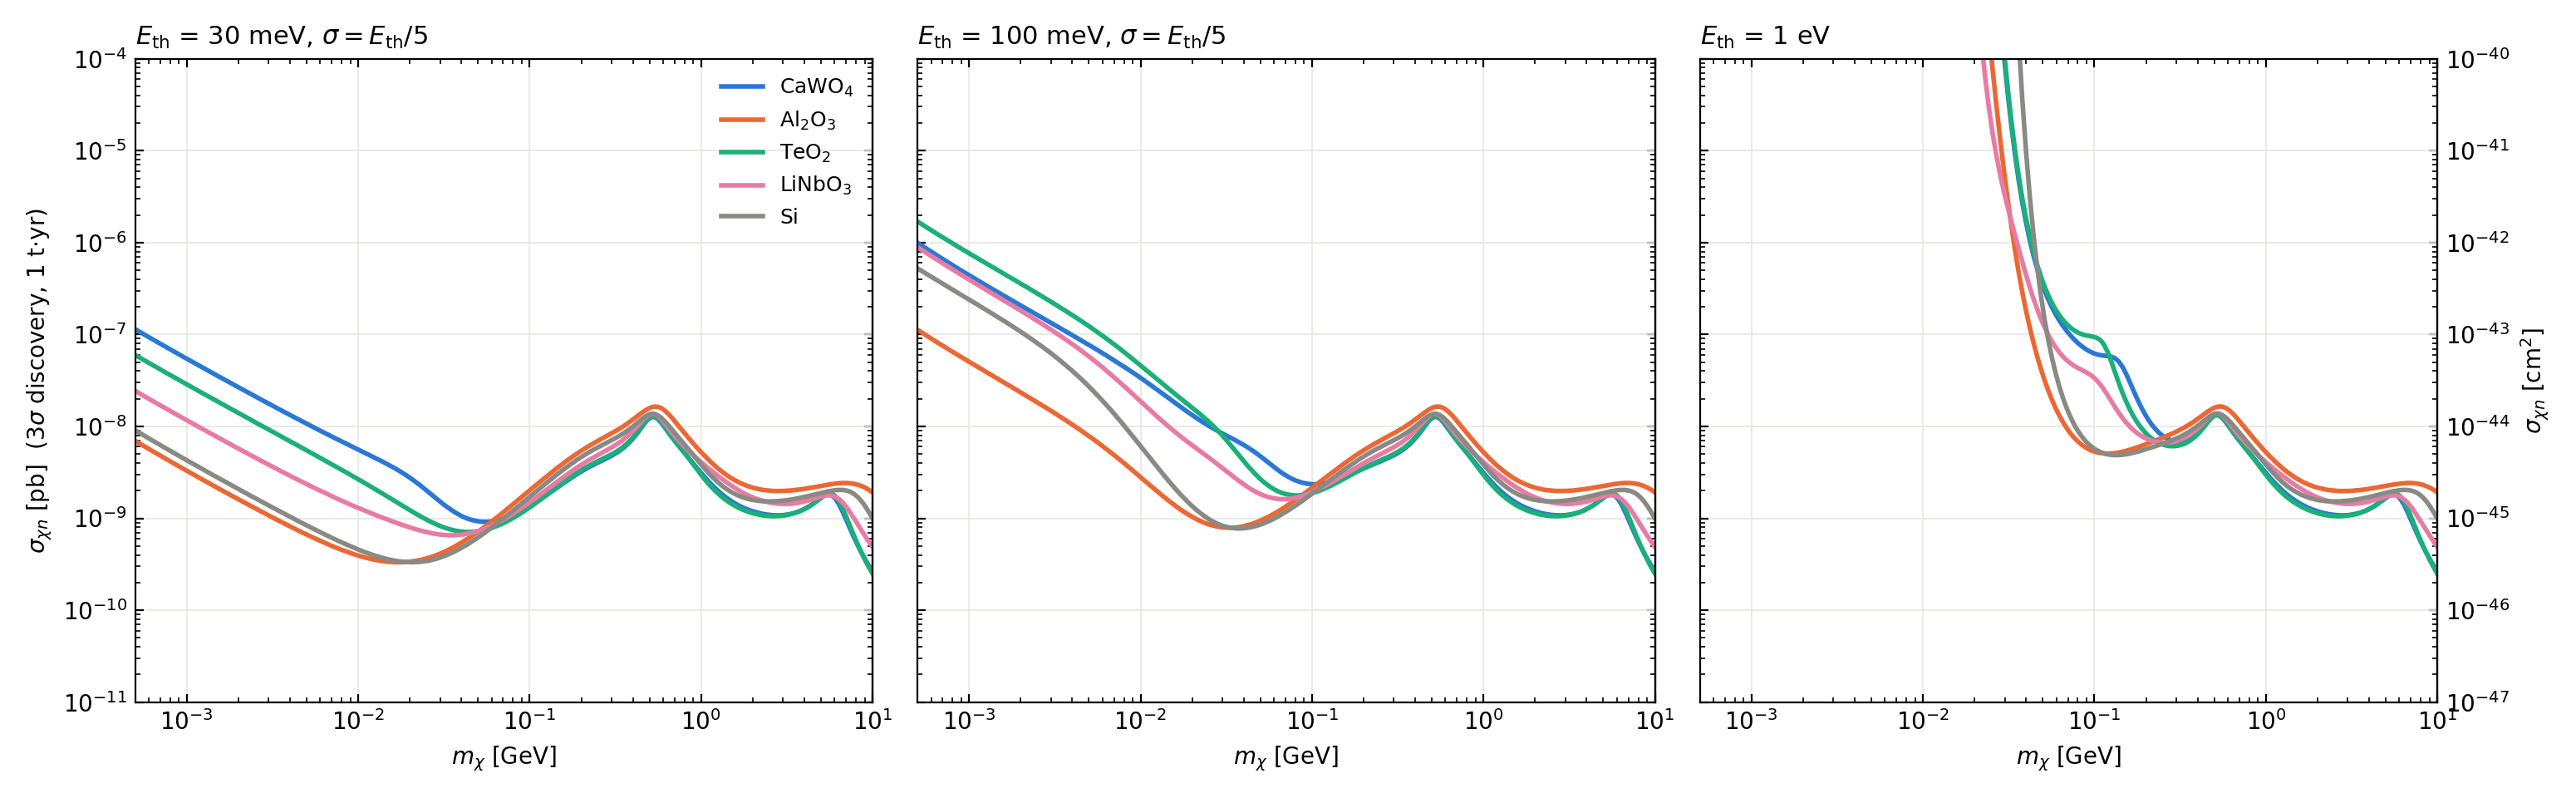
\includegraphics[width=\textwidth]{fog_all_materials.png}
\caption{3$\sigma$ discovery limits (1\,t$\cdot$yr) for five crystals at
$\Eth=30$\,meV and 100\,meV (with $\sigma_E=\Eth/5$) and at 1\,eV.}
\label{fig:fog_all}
\end{figure}
Below 5\,MeV at 30\,meV, Al$_2$O$_3$ is best. Relative to it, Si is weaker by $1.3\times$,
LiNbO$_3$ by $3.6\times$, TeO$_2$ by $8\times$ and CaWO$_4$ by $16\times$. Above 100\,MeV,
TeO$_2$ and CaWO$_4$ lead by 1.3--1.8$\times$, thanks to the coherent $A^2$
(Fig.~\ref{fig:fog_all}). The multiphonon gap tracks the heaviest, softest atom: CaWO$_4$ 38,
TeO$_2$ 16, LiNbO$_3$ 8, Si 5.6, Al$_2$O$_3$ 2.9.

\subsection{Daily modulation}
\label{sec:res_dir}
\begin{figure}[h]
\centering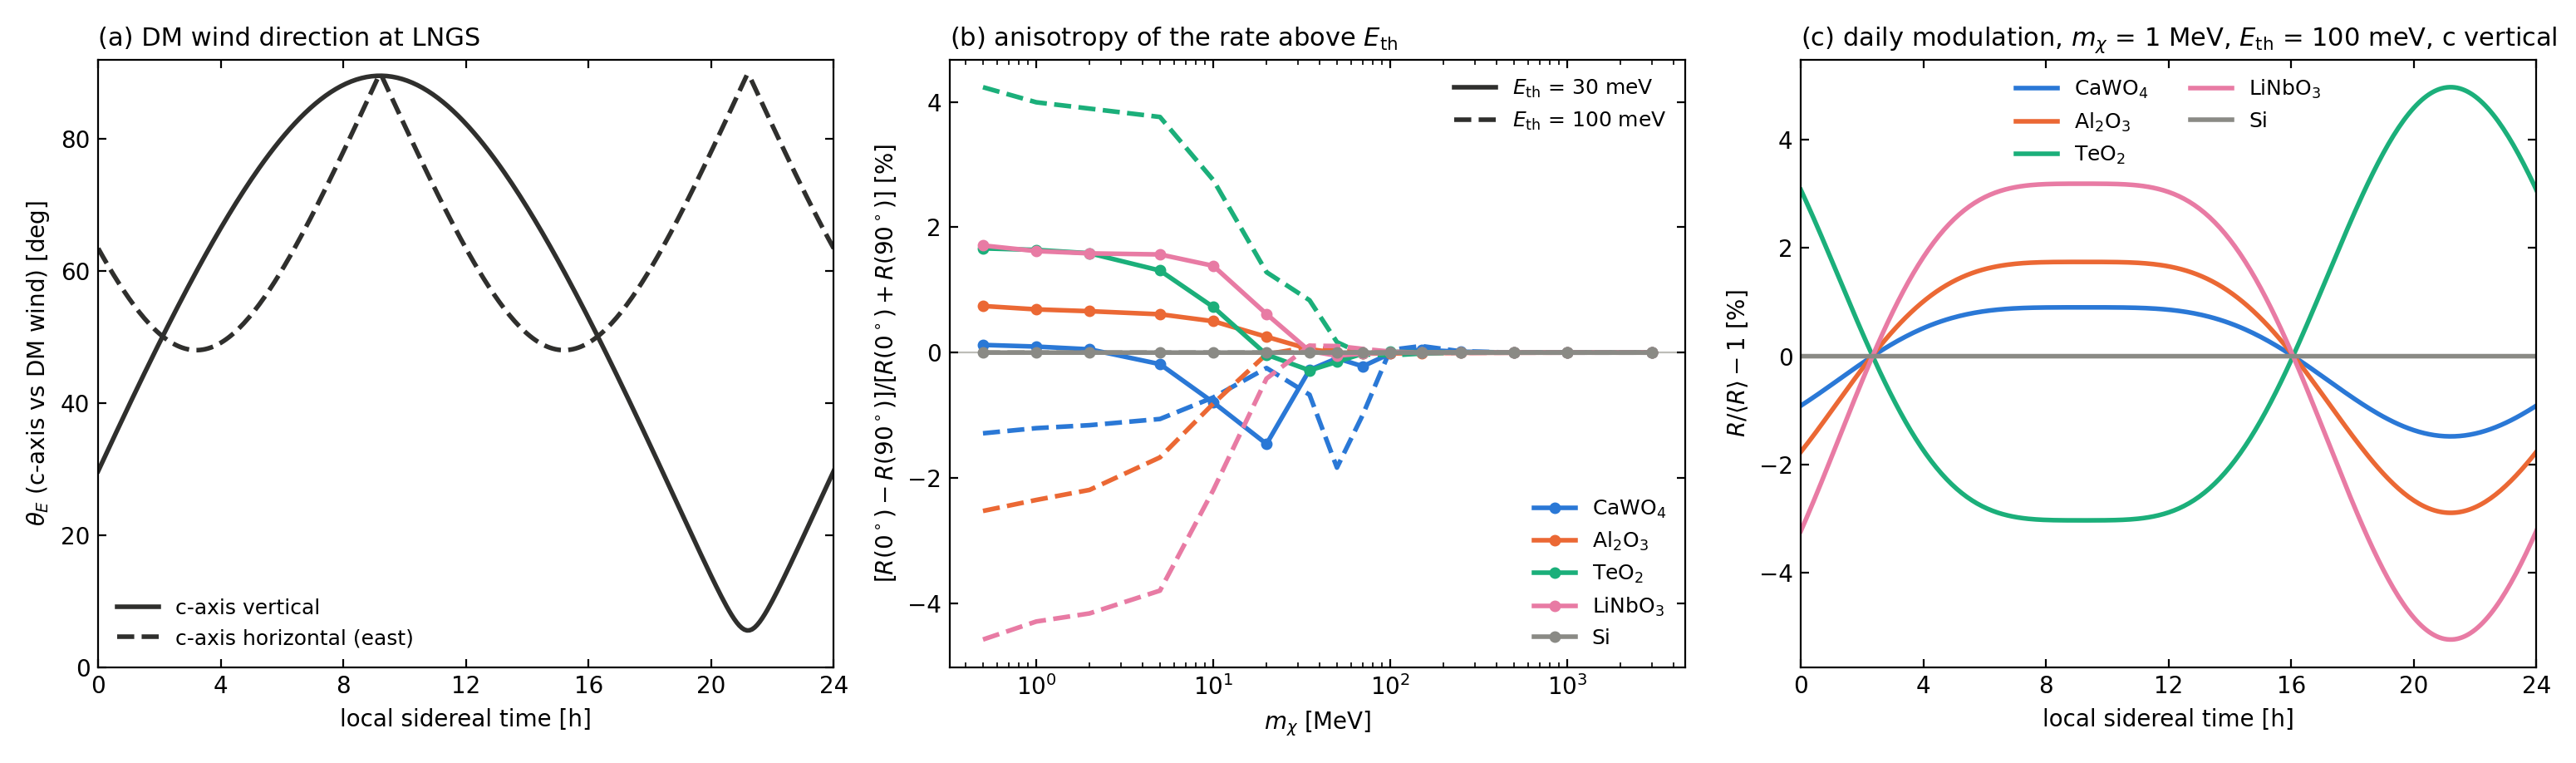
\includegraphics[width=\textwidth]{directional_modulation.png}
\caption{(a) $\theta_E$ over a sidereal day at LNGS. (b) Anisotropy
$[R(0^\circ)-R(90^\circ)]/[R(0^\circ)+R(90^\circ)]$ vs mass at 30\,meV (solid) and 100\,meV
(dashed). (c) Daily modulation at 1\,MeV, 100\,meV, for a vertical $c$ axis.}
\label{fig:dir}
\end{figure}
The signed anisotropy at 1\,MeV (30 / 100\,meV) is:
\begin{itemize}
  \item CaWO$_4$: $+0.1\%$ / $-1.2\%$;
  \item Al$_2$O$_3$: $+0.7\%$ / $-2.4\%$;
  \item TeO$_2$: $+1.6\%$ / $+4.0\%$;
  \item LiNbO$_3$: $+1.6\%$ / $-4.3\%$;
  \item Si: 0.
\end{itemize}
The effect disappears above about 50\,MeV, where the impulse regime is isotropic. The sign
reversal with threshold reflects the Poisson structure of Eq.~\eqref{eq:poisson}:
\begin{itemize}
  \item near threshold the rate weights $\hat T_1\propto D/\omega$, favouring the softer
  direction;
  \item above the top optical phonon, events need several phonons from the top of the
  spectrum, favouring the stiffer direction.
\end{itemize}

\paragraph{Benchmark against Stratman \& Lin.}
With their conventions ($v_E=240$, $v_{\rm esc}=500$\,km/s, no resolution, $c\parallel\vec v_E$
at $t=0$, $\theta_e=42^\circ$, $A_{\rm mod}=|R(0)-\avg R|/\avg R$), Al$_2$O$_3$ at 10\,MeV gives
$A_{\rm mod}=2.7$, 5.3 and 7.4\% for $\Eth=120$, 200 and 300\,meV, with a maximum of 9.8\% at
3--5\,MeV. Their result is up to about 11\%. Magnitude, threshold dependence and mass range
agree; the remaining 30\% at 10\,MeV is consistent with differences in the inputs.

\subsection{Comparison with CRESST}
\label{sec:res_cresst}
\begin{figure}[h]
\centering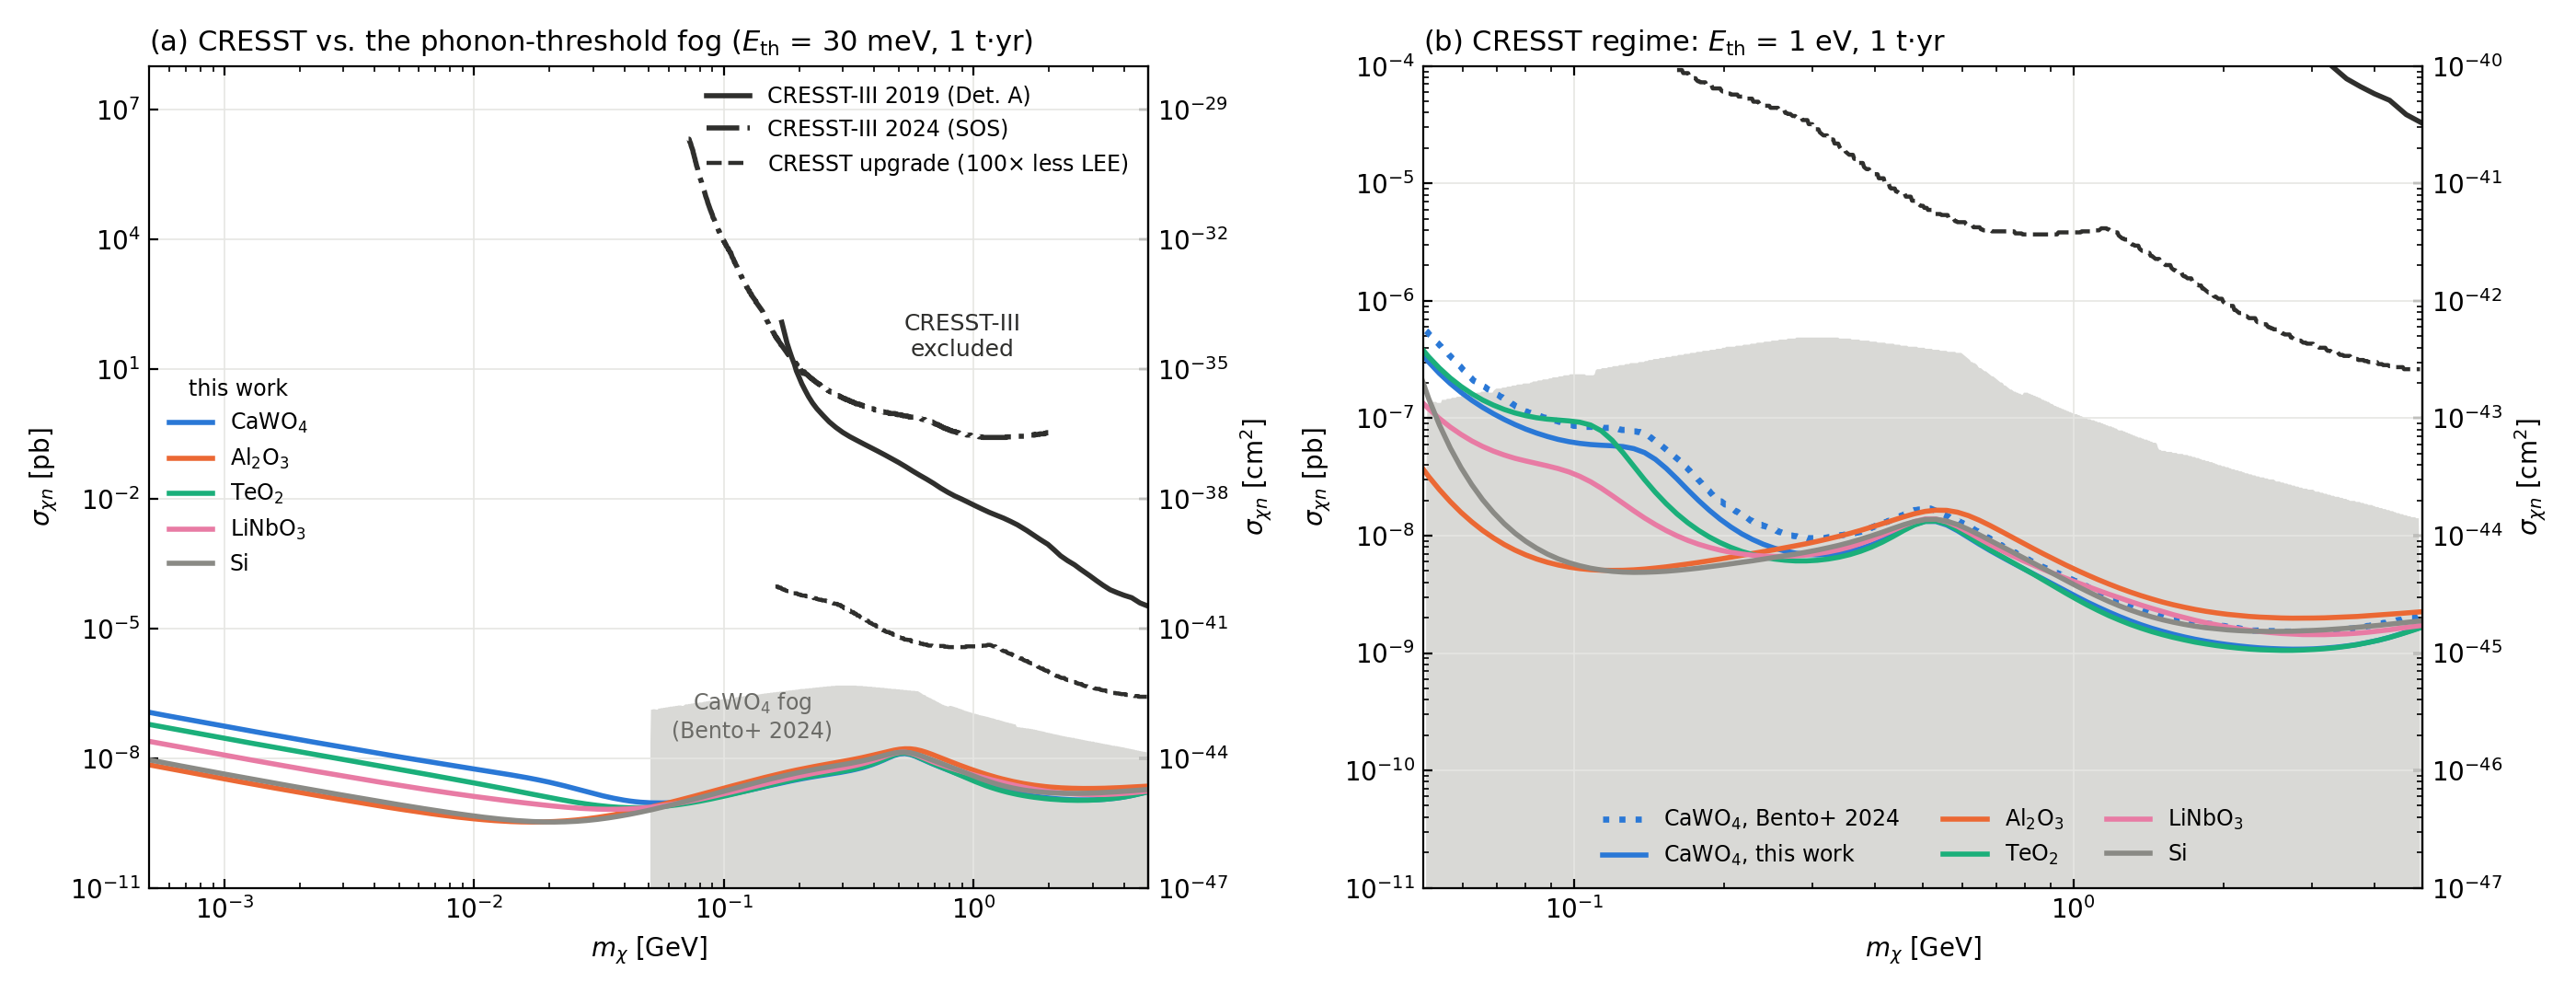
\includegraphics[width=\textwidth]{fog_vs_cresst.png}
\caption{(a) CRESST-III limits (2019, published data; 2024 SOS, digitized) and the upgrade
projection with 100$\times$ less low-energy excess, against the discovery limits of this work at
30\,meV. Grey: CaWO$_4$ fog of Bento \emph{et al.}\ (2024). (b) $\Eth=1$\,eV: this work vs
Bento \emph{et al.}\ for CaWO$_4$ (dotted).}
\label{fig:cresst}
\end{figure}
\begin{itemize}
  \item At 1\,GeV, CRESST-III lies about six orders of magnitude above the neutrino-limited
  region, and the upgrade about two. CRESST is limited by its low-energy excess.
  \item A 30\,meV phonon threshold opens the region from 0.5\,MeV upward, which CRESST
  (lowest mass 73\,MeV) does not reach. In that region Al$_2$O$_3$ and Si outperform
  CaWO$_4$ by more than an order of magnitude.
  \item At 1\,eV our CaWO$_4$ curve reproduces the shape of Bento \emph{et al.}, including the
  $^8$B feature at 0.5\,GeV, and lies a factor 0.61--0.78 below it.
\end{itemize}

\subsection{Background or fog?}
\begin{figure}[h]
\centering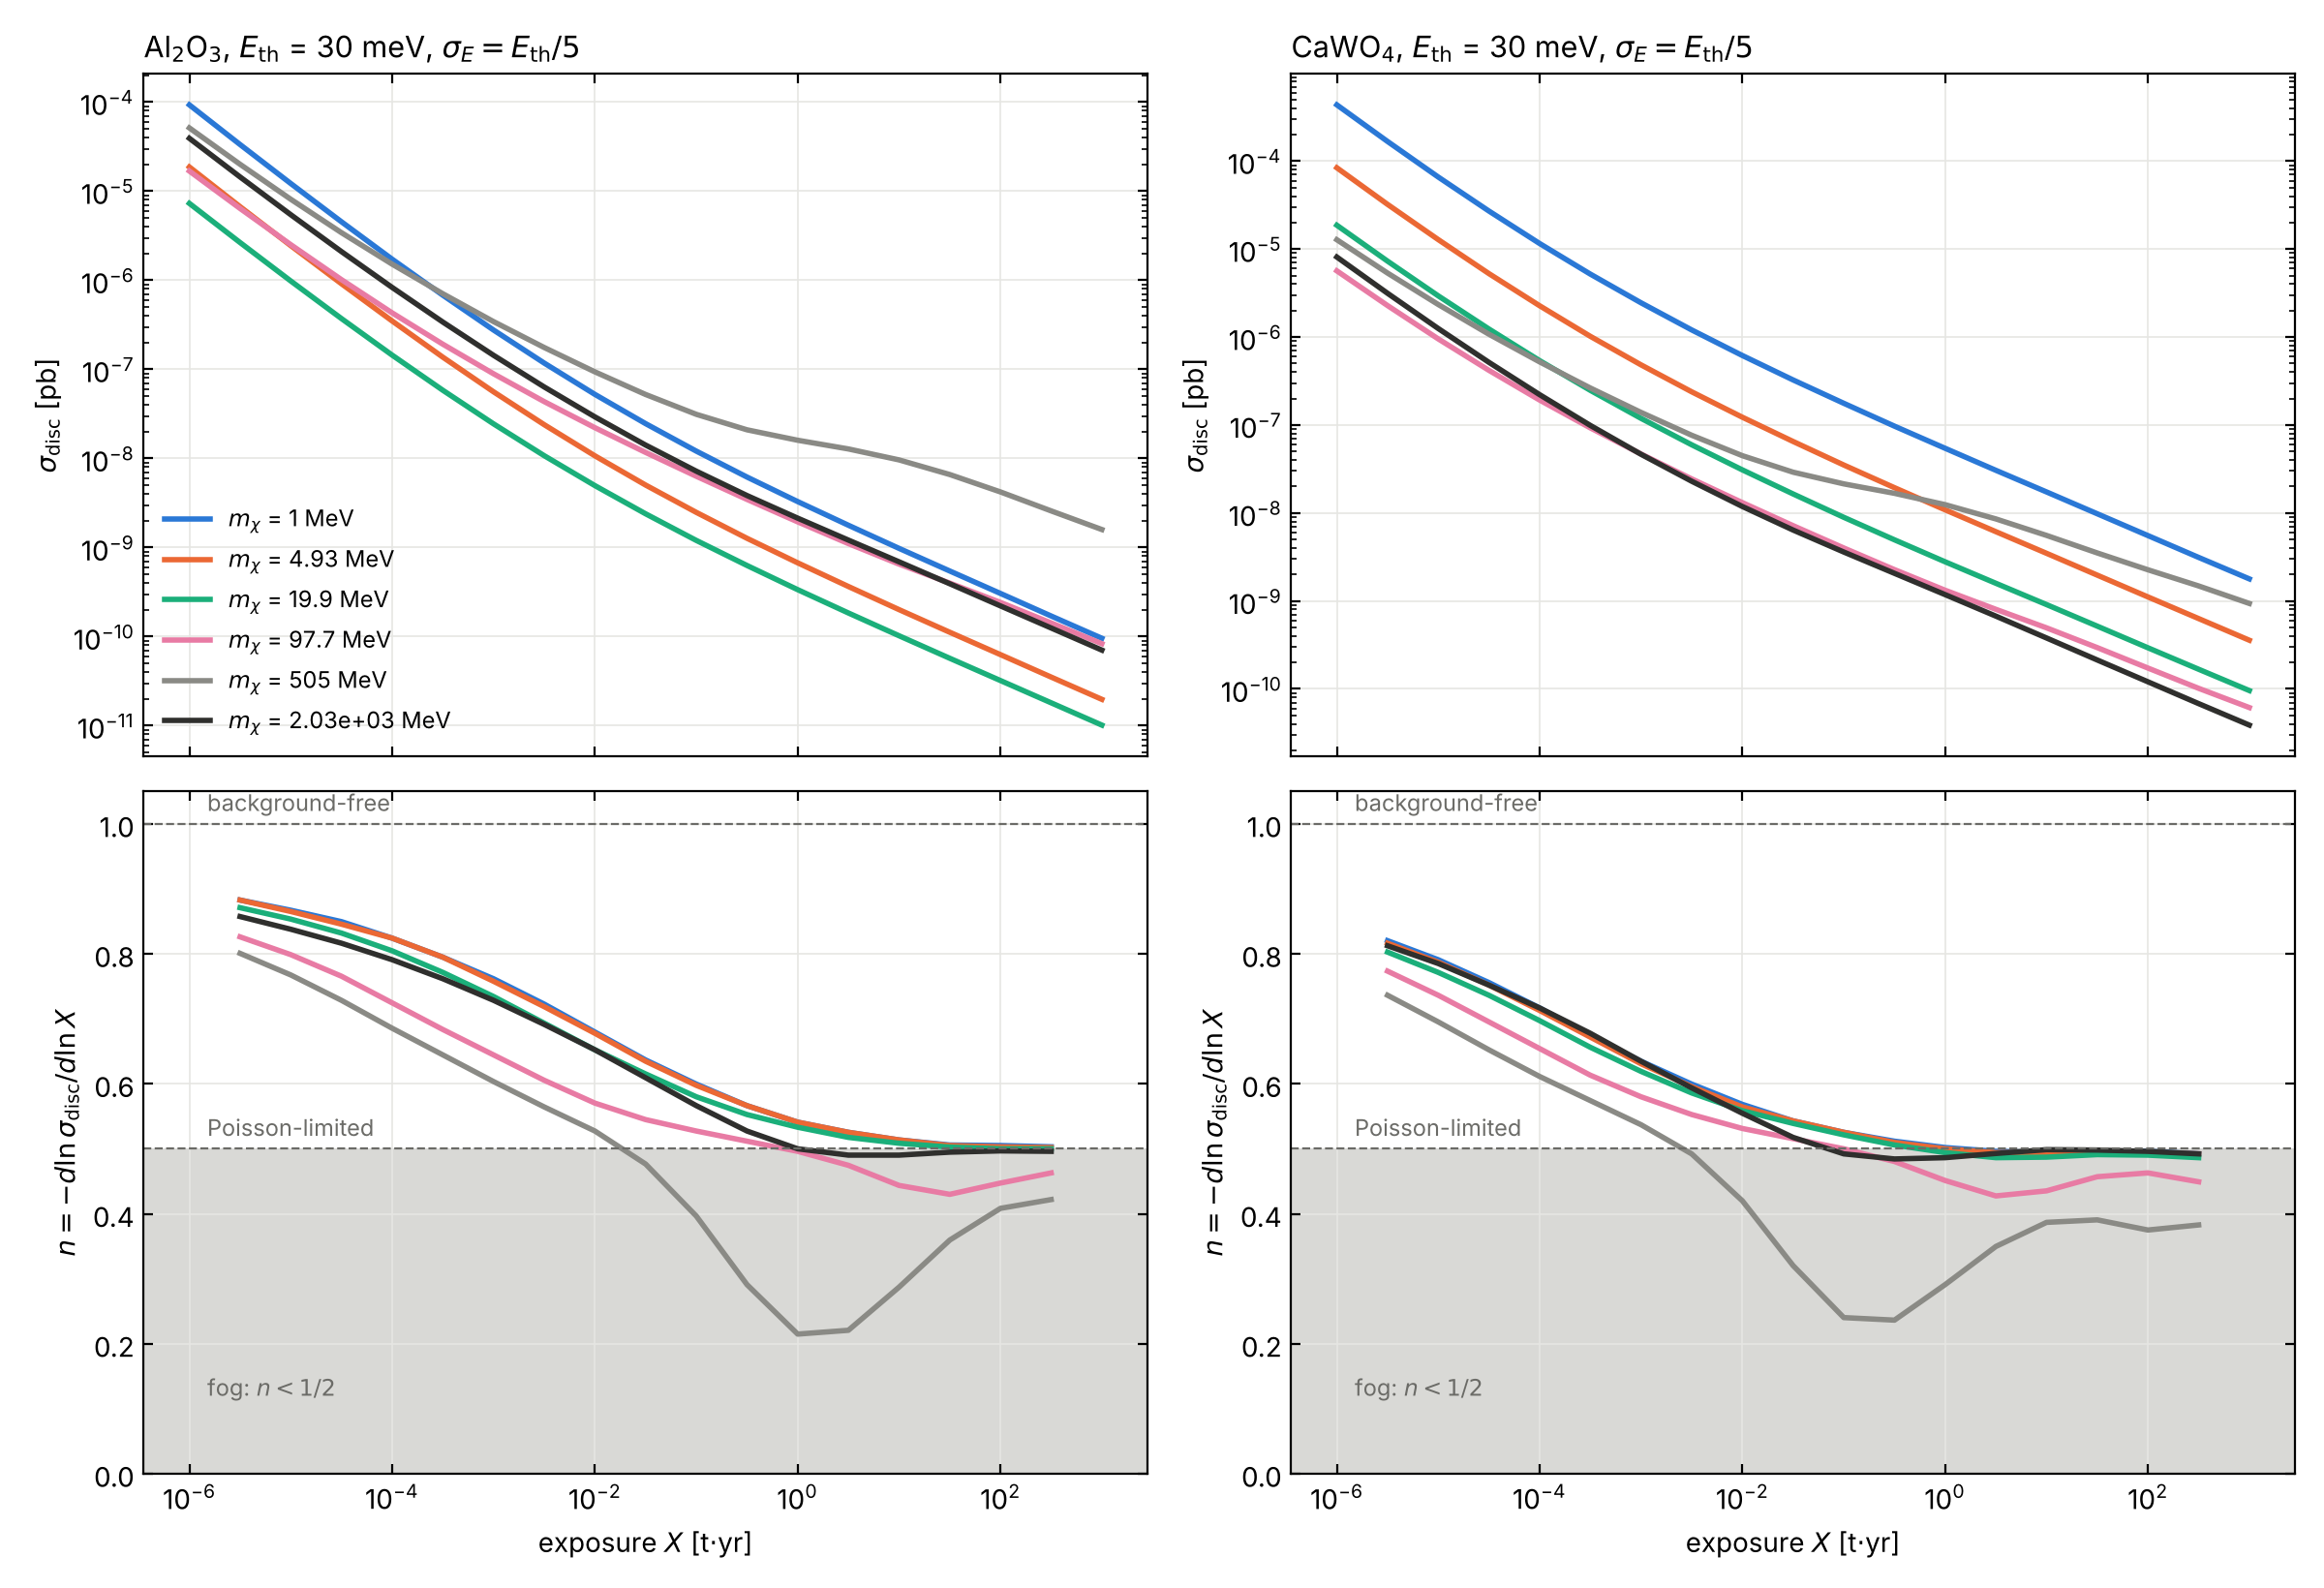
\includegraphics[width=0.92\textwidth]{exposure_scan.png}
\caption{Discovery cross section (top) and fog index $n=-\dd\ln\sigma/\dd\ln X$ (bottom) vs
exposure, at $\Eth=30$\,meV with $\sigma_E=\Eth/5$. The grey band is the fog, $n<\frac12$.}
\label{fig:scan}
\end{figure}
Above 30\,meV, Al$_2$O$_3$ sees $3.7\times10^3$ neutrino events per t$\cdot$yr (pp 52\%,
$^7$Be 37\%, $^8$B 3\%); CaWO$_4$ sees $2.8\times10^4$. Figure~\ref{fig:scan} shows:
\begin{itemize}
  \item \textbf{1--20\,MeV}: $n\to0.50$ and never lower. The multiphonon DM spectrum has a
  component outside the span of the pp and $^7$Be CEvNS spectra
  ($\bm\varepsilon_\perp\neq0$, Sec.~\ref{sec:fogindex}). DM remains discoverable, and the
  reach improves as $X^{-1/2}$.
  \item \textbf{About 100\,MeV}: mild saturation ($n\simeq0.43$--0.47) above a few t$\cdot$yr.
  \item \textbf{About 0.5\,GeV}: a genuine fog, $n\simeq0.2$--0.4, where the DM spectrum is
  nearly degenerate with $^8$B.
\end{itemize}
Representative values for Al$_2$O$_3$:
$\sigma_{\rm disc}(1\,{\rm MeV})=2.8\times10^{-43}$\,cm$^2$ at 1\,kg$\cdot$yr and
$3.3\times10^{-45}$\,cm$^2$ at 1\,t$\cdot$yr.

To reach the neutrino-limited regime, a detector needs:
\begin{itemize}
  \item a threshold of about 30\,meV with $\sigma_E\approx6$\,meV;
  \item an exposure of about 0.1--1\,t$\cdot$yr (Al$_2$O$_3$);
  \item non-neutrino backgrounds below about 0.01 events/(kg$\cdot$day) above threshold.
\end{itemize}
The last requirement is many orders of magnitude below today's low-energy excess.

%==============================================================================
\section{Why the lattice response must be known precisely}
\label{sec:precision}
%==============================================================================
\subsection{Power-law sensitivity of the multiphonon rate}
By Eq.~\eqref{eq:poisson}, the $n$-phonon contribution is
${\rm Pois}(n;\lambda)\hat T_n(\omega)$ with $\lambda=q^2\avg{1/\omega}/2m_d$. Holding the shape
$\hat T_1$ fixed and varying the moment $\avg{1/\omega}$,
\begin{equation}
  \frac{\partial\ln S_{d,n}}{\partial\ln\avg{1/\omega}}=n-\lambda .
  \label{eq:sens}
\end{equation}
At low DM mass $q$ is small and $\lambda\ll1$, so the $n$-phonon rate scales as
$\avg{1/\omega}^n$. A deposit above threshold needs at least
\begin{equation}
  n_{\min}=\left\lceil\frac{\Eth}{\omega_{\max}}\right\rceil
\end{equation}
phonons, where $\omega_{\max}$ is the top of the phonon spectrum. The rate above threshold is
therefore $\propto\avg{1/\omega}^{n_{\min}}$. For example, a 20\% error in $\avg{1/\omega}$
(the size of the acoustic-slope errors found in the CaWO$_4$ and Si force constants) changes a
three-phonon rate by $1.2^3\simeq1.7$. That is exactly the size of the change observed when the
CaWO$_4$ tensor was corrected ($1.5$--$1.65\times$).

Because $\avg{1/\omega}$ is dominated by the softest modes (87\% of the tungsten value comes
from 2--10\,meV), the low-energy acoustic branches control the low-mass reach. Those are the
branches most affected by supercell size, imaginary modes and DFT softening.

\subsection{Sensitivity to the top of the spectrum}
The support of $\hat T_n$ ends at $n\,\omega_{\max}$. When $\Eth$ is close to a multiple of
$\omega_{\max}$, a small shift of the highest optical branch changes $n_{\min}$ by one, and the
rate by a factor of order $\lambda$, which can be orders of magnitude at low mass. The shape of
$D(\omega)$ near the band top sets how the rate falls across threshold. This is why the
CaWO$_4$ reach at $\Eth=0.1$\,eV, right at the 110\,meV optical peak, changes by $1.4\times$
when the edge is smeared by 20\,meV resolution.

\subsection{Discrimination depends on the spectral shape}
Section~\ref{sec:fogindex} shows that DM can be separated from neutrinos only through the
component of its spectrum orthogonal to the neutrino templates. Both spectra are produced by
the same $S(\qv,\omega)$, with different weights in $q$:
\begin{itemize}
  \item DM: $q\lesssim2\mchi v$, weighted by $\eta(v^*)$;
  \item CEvNS: $q\lesssim2E_\nu$, weighted by the neutrino spectrum.
\end{itemize}
The orthogonal component, and with it the $n=\frac12$ behaviour in Fig.~\ref{fig:scan}, is a
property of the lattice response. If $S$ is uncertain, its uncertainty enters the likelihood
as a further nuisance direction that moves signal and background together. Any part of the DM
spectrum that this nuisance can mimic becomes degenerate. That converts a Poisson background
into a fog, $n<\frac12$, even where the neutrino fluxes alone would not. An imprecise $S$
therefore does more than shift the curves: it can change the scaling of the reach with
exposure.

\subsection{Further consequences}
\begin{itemize}
  \item \textbf{Target selection.} The 16$\times$ spread between materials at low mass and the
  2.9--38$\times$ multiphonon gap are properties of $D_d(\omega)$.
  \item \textbf{Directionality} requires the per-atom anisotropy of the DOS tensor, and
  therefore the eigenvectors, not only the frequencies. Its sign flips with threshold.
  \item \textbf{Neutrino background.} pp and $^7$Be CEvNS populate the same meV--eV window
  through the same $S$, so the background prediction inherits the same uncertainties.
\end{itemize}

\subsection{Sources of uncertainty and how to control them}
\begin{itemize}
  \item \textbf{Force constants}: supercell convergence (soft TA branches, imaginary pockets),
  DFT functional (acoustic softening), missing LO--TO correction. \emph{Control:} converged
  supercells, Born charges, comparison with measured sound speeds and inelastic neutron
  scattering DOS.
  \item \textbf{Model approximations}: harmonic and $T=0$ approximations; incoherent
  approximation (invalid for $q\lesssim$ few keV); impulse switch at $\lambda=16$.
  \emph{Control:} coherent single-phonon calculations at low $q$; anharmonic corrections where
  $n$ is large.
  \item \textbf{Propagation}: include a parametrized uncertainty on $S$ (for example, the scale
  of $\avg{1/\omega}$ and of the acoustic slopes) as a nuisance in the likelihood. This
  quantifies how much of the low-mass reach is robust.
\end{itemize}

%==============================================================================
\section{Conclusions}
%==============================================================================
\begin{enumerate}
  \item The rewritten pipeline reproduces the free-nucleus limit to 0.1\% and the
  phonon sum rules to 1\%, for five materials. It runs in seconds.
  \item Multiphonon emission dominates the low-mass reach; ignoring it costs up to $38\times$
  in CaWO$_4$. For thresholds of tens of meV, Al$_2$O$_3$ and Si are the best targets below
  50\,MeV, while heavy targets win above 100\,MeV.
  \item In the phonon regime (1--20\,MeV) the neutrino background is a Poisson background,
  not a fog. DM is discoverable through it, and the reach improves as $X^{-1/2}$. A genuine
  fog appears only near 0.5\,GeV ($^8$B), with mild saturation from about 100\,MeV.
  \item CRESST is 2--6 orders of magnitude above this regime and limited by its low-energy
  excess. Reaching the neutrino-limited phonon regime requires thresholds of about 30\,meV
  and backgrounds below about 0.01/(kg$\cdot$day).
  \item Anisotropic crystals show a percent-level sidereal modulation (up to about 10\% at
  higher thresholds) below about 50\,MeV, with a threshold-dependent phase. It is a tool to
  confirm the DM origin of a signal, not to discover one.
  \item All these conclusions depend on $S(\qv,\omega)$. The multiphonon rate scales as a
  power of the phonon moments, and the separation of DM from neutrinos depends on the
  spectral shape. Converged, experimentally validated phonon inputs, and their uncertainty
  propagated into the likelihood, are therefore required for robust low-mass projections.
  The most urgent case is CaWO$_4$.
\end{enumerate}

\section*{References}
\small
\begin{enumerate}[label={[\arabic*]},leftmargin=*]
\item CRESST Collaboration, Commun.\ Phys.\ (2025), doi:10.1038/s42005-025-02476-5.
\item A.~Bento \emph{et al.}, Eur.\ Phys.\ J.\ C \textbf{84}, 1118 (2024).
\item B.~Campbell-Deem, S.~Knapen, T.~Lin, E.~Villarama, Phys.\ Rev.\ D \textbf{106}, 036019 (2022).
\item S.~Knapen, J.~Kozaczuk, T.~Lin, Phys.\ Rev.\ D \textbf{105}, 015014 (2022) [DarkELF].
\item C.~Stratman, T.~Lin, arXiv:2411.03433.
\item S.~Griffin, S.~Knapen, T.~Lin, K.~M.~Zurek, Phys.\ Rev.\ D \textbf{98}, 115034 (2018).
\item C.~A.~J.~O'Hare, Phys.\ Rev.\ Lett.\ \textbf{127}, 251802 (2021).
\item A.~H.~Abdelhameed \emph{et al.} (CRESST), Phys.\ Rev.\ D \textbf{100}, 102002 (2019).
\end{enumerate}

\appendix
\section{Program inventory (NuFog\_v2)}
\small
\begin{tabularx}{\textwidth}{>{\raggedright\arraybackslash}p{7.2cm}X}
\toprule
Program & Purpose\\
\midrule
\texttt{config.py} & Settings (material via \texttt{NUFOG\_MATERIAL}, grids, $n_{\max}$, $\Eth$, exposure, resolution, halo)\\
\texttt{nufog\_core.py} & $S(\qv,\omega)$, DM and CEvNS rates, binning, resolution\\
\texttt{likelihood.py} & Asimov $q_0$ with Newton profile\\
\texttt{step1}--\texttt{step4}, \texttt{run\_all.py} & Neutrino spectra, DM matrix, discovery curves, plot\\
\texttt{check\_normalization.py}, \texttt{compare\_v1.py} & Free-nucleus benchmark; v1 vs v2\\
\texttt{diagnose\_spectra.py}, \texttt{compare\_materials.py} & Spectra diagnostics; material comparison\\
\texttt{directional.py}, \texttt{check\_directional.py} & $R(\mchi,\theta_E)$; isotropic-limit check\\
\texttt{daily\_modulation.py}, \texttt{directional\_summary.py}, \texttt{plot\_directional.py} & Sidereal modulation and figure\\
\texttt{compare\_stratman\_lin.py} & Benchmark against Stratman \& Lin\\
\texttt{plot\_fog\_cresst.py}, \texttt{literature/} & CRESST comparison (published and digitized curves)\\
\texttt{exposure\_scan.py}, \texttt{plot\_exposure\_scan.py} & Fog index vs exposure\\
\bottomrule
\end{tabularx}
\end{document}
